\documentclass[11pt,oneside]{article}
\usepackage[T1]{fontenc}
\usepackage[utf8]{inputenc}
%\DeclareUnicodeCharacter{00A0}{ }
\usepackage[adobe-utopia]{mathdesign}

\usepackage{amsmath}
\usepackage[francais]{babel}
\usepackage[dvips]{graphicx}
%\usepackage{here}
\usepackage{framed}
\usepackage[normalem]{ulem}
\usepackage{fancyhdr}
\usepackage{titlesec}
\usepackage{vmargin}

\usepackage{amsmath}
\usepackage{ifthen}
\usepackage{multirow}
\usepackage{multicol} % Portions de texte en colonnes

%\usepackage{xltxtra} % Logo XeLaTeX
%\usepackage{pst-solides3d}
\usepackage{color}
%\usepackage{colortbl}
\usepackage{titletoc} % Pour la mise en forme de la table des matières

%\usepackage[crop=off]{auto-pst-pdf}
%\usepackage{bclogo}


%\usepackage{longtable}
%\usepackage{flafter}%floatants après la référence
%\usepackage{pst-solides3d}
%\usepackage{pstricks}
%\usepackage{minitoc}
%\setcounter{minitocdepth}{4}
%\usepackage{draftcopy}% "Brouillon"
%\usepackage{floatflt}
%\usepackage{psfrag}
%\usepackage{listings} % Permet d'insérer du code de programmation
%\usepackage{lmodern}
%\usepackage[adobe-utopia,uppercase=upright,greeklowercase=upright]{mathdesign}
%\usepackage{minionpro}
%\usepackage{pifont}
%\usepackage{amssymb}
%\usepackage[francais]{varioref}

\setmarginsrb{1.5cm}{1cm}{1cm}{1.5cm}{1cm}{1cm}{1cm}{1cm}

\definecolor{gris25}{gray}{0.75}
\definecolor{bleu}{RGB}{18,33,98}
\definecolor{bleuf}{RGB}{42,94,171}
\definecolor{bleuc}{RGB}{231,239,247}
\definecolor{rougef}{RGB}{185,18,27}
\definecolor{rougec}{RGB}{255,230,231}
\definecolor{vertf}{RGB}{103,126,82}
\definecolor{vertc}{RGB}{220,255,191}
\definecolor{violetf}{RGB}{112,48,160}
\definecolor{violetc}{RGB}{230,224,236}
\definecolor{jaunec}{RGB}{220,255,191}

\usepackage{style/schemabloc}
%Si le boolen xp est vrai : compilation pour xabi
%Sinon compilation Damien
\newboolean{xp}
\setboolean{xp}{true}

\newboolean{prof}
\setboolean{prof}{true}

\def\xxtitre{\ifthenelse{\boolean{xp}}{
CI 2 -- SLCI : Étude du comportement des Systèmes Linéaires Continus Invariants}{
}}

\def\xxsoustitre{\ifthenelse{\boolean{xp}}{
Exercice de colle}{
}}


\def\xxauteur{\ifthenelse{\boolean{xp}}{
\noindent 2013 -- 2014 \\
Florestan \textsc{Mathurin}}{
}}


\def\xxpied{\ifthenelse{\boolean{xp}}{
CI 2 : SLCI\\
Exercice de colle \ifthenelse{\boolean{prof}}{P}{E}%
}{
}}

\usepackage[%
    pdftitle={SLCI - Systèmes du second ordre},
    pdfauthor={Xavier Pessoles},
    colorlinks=true,
    linkcolor=blue,
    citecolor=magenta]{hyperref}



\usepackage{pifont}
\sloppy
\hyphenpenalty 10000


\begin{document}






% \makeatletter \let\ps@plain\ps@empty \makeatother
%% DEBUT DU DOCUMENT
%% =================




%------------- En tetes et Pieds de Pages ------------


\pagestyle{fancy}
\ifthenelse{\boolean{xp}}{%
\renewcommand{\headrulewidth}{0pt}}{%
\renewcommand{\headrulewidth}{0.2pt}} %pour mettre le trait en haut
%\renewcommand{\headrulewidth}{0.2pt}

\fancyhead{}
\fancyhead[L]{%
\ifthenelse{\boolean{xp}}{%
\noindent\begin{minipage}[c]{2.6cm}%

\includegraphics[width=2cm]{png/logo_ptsi.png}%
\end{minipage}%
}{%
\footnotesize{\textit{\textsf{Lycée François Premier}}}
}}

\ifthenelse{\boolean{xp}}{%
\fancyhead[C]{\rule{12cm}{.5pt}}}{
}


\fancyhead[R]{%
\noindent\begin{minipage}[c]{3cm}
\begin{flushright}
\footnotesize{\textit{\textsf{Sciences Industrielles \\ de l'ingénieur}}}%
\end{flushright}
\end{minipage}
}


\ifthenelse{\boolean{xp}}{%
\fancyhead[C]{\rule{12cm}{.5pt}}}{
}

\renewcommand{\footrulewidth}{0.2pt}

\fancyfoot[C]{\footnotesize{\bfseries \thepage}}
\fancyfoot[L]{%
\begin{minipage}[c]{.2\linewidth}
\noindent\footnotesize{{\xxauteur}}
\end{minipage}
\ifthenelse{\boolean{xp}}{}{%
\begin{minipage}[c]{.15\linewidth}

\includegraphics[width=2cm]{png/logoCC.png}
\end{minipage}}
}


\fancyfoot[R]{\footnotesize{\xxpied}}



\begin{center}
 \Large\textsc{\xxtitre}
\end{center}

\begin{center}
 \large\textsc{\xxsoustitre}
\end{center}

%\vspace{.5cm}

\begin{center}
 \large\textsc{Unité dentaire}
\end{center}

%\begin{flushright}
%\textit{D'après ressources d'Alain Caignot.}
%\end{flushright}




\subsection*{Cours}
\begin{itemize}
\item Donner la fonction de transfert d'un système du second ordre
\item Donner l'expression de la pseudo-période
\item Donner l'expression du dépassement
\item Donner l'allure de la réponse indicielle en fonction de la valeur du
coefficient d'amortissement
\end{itemize}


\section*{Unité dentaire}
\textit{(Selon le concours E3A PSI 2007)}
\vspace{0.25cm}


\begin{minipage}[c]{.6\linewidth}
Le support de l'étude est une "unité dentaire" dont on donne un extrait du cahier des charges fonctionnel. Cet équipement a été conçu et réalisé dans le but d'une adaptabilité maximale aux différentes méthodes de travail des chirurgiens dentistes. Son ergonomie, sa maniabilité, son design, sa fiabilité en font une "unité universelle". Sa conception est modulaire avec une technologie avancée.

Le chirurgien dentiste possède une pédale et un pupitre de commande, qui lui permet de monter ou descendre verticalement le corps du patient, de l'incliner plus ou moins, et de positionner sa tête. Le patient pouvant prendre une position spatiale pertinente, tous les actes médicaux sont facilités.
\end{minipage}\hfill
\begin{minipage}[c]{.35\linewidth}
\begin{center}
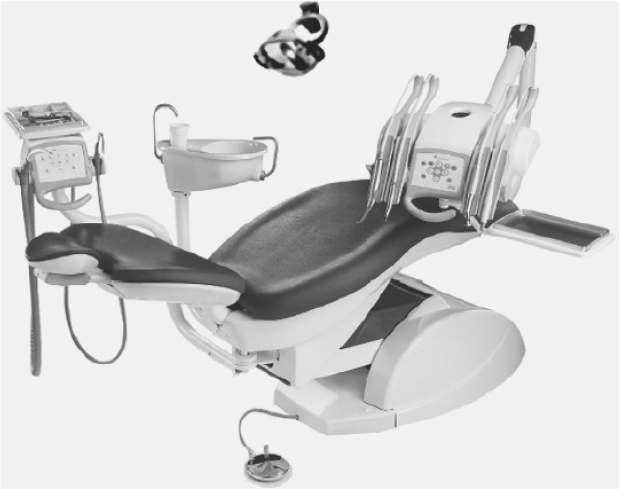
\includegraphics[width=.9\textwidth]{png/fig1}
\end{center}
\end{minipage}

\begin{center}
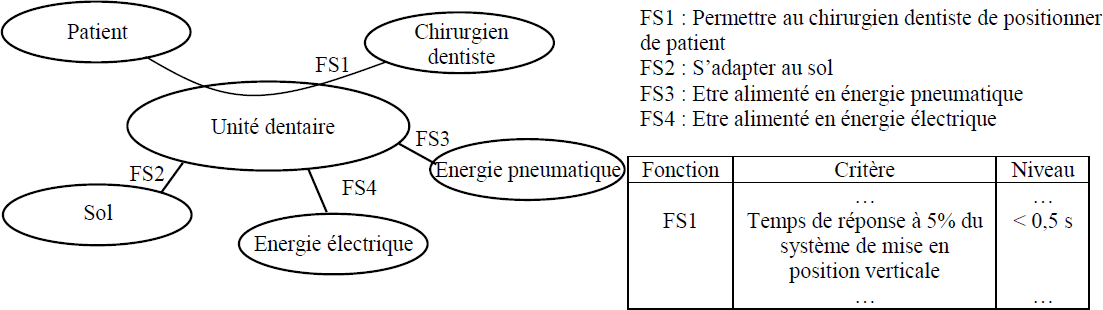
\includegraphics[width=.9\textwidth]{png/fig2}
\end{center}

On s'intéresse dans ce sujet au critère de la FS1 concernant le temps de réponse du système permettant de mettre en position verticale le patient. 

Pour régler le patient en position verticale, le chirurgien dentiste appuie sur une pédale, plus ou moins fort. Un moteur électrique se met en route, sa vitesse de rotation dépend de l'appui plus ou moins profond du chirurgien dentiste sur la pédale. La vitesse de rotation du moteur est diminuée par un réducteur à engrenages. En sortie du réducteur à engrenages se trouve une vis dont la rotation $\Omega_v(p)$ entraîne, par un système vis-écrou, la translation du siège en hauteur. L'ensemble peut se représenter par le schéma bloc suivant. Le composant de fonction de transfert $C(p)$ est un correcteur :


\begin{center}
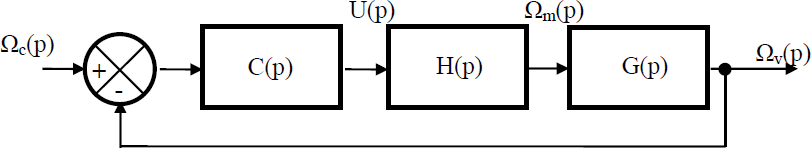
\includegraphics[width=.6\textwidth]{png/fig3}
\end{center}

\subparagraph{}
\textit{Déterminer le nom des composants qui réalisent les fonctions $H(p)$ et $G(p)$.}

\subparagraph{}
\textit{Déterminer la fonction de transfert en boucle fermée du système $\dfrac{\Omega_v(p)}{\Omega_c(p)}$.}

Les équations du moteur utilisé sont les suivantes :
$$
u(t)=e(t)+Ri(t)+K\dfrac{di(t)}{dt} \quad e(t) = k_e \omega_m(t) \quad J\cdot\dfrac{d\omega_m(t)}{dt} = C_m(t)-f\omega_m(t) \quad C_m(t)=k_m \cdot i(t)
$$

On note $u(t)$ tension du moteur, $e(t)$, la force contre électro motrice du moteur, $i(t)$ l'intensité dans le moteur, $C_m(t)$ le couple exercé par le moteur et $\omega_m(t)$ la vitesse angulaire du moteur. Les grandeurs physiques $R$, $L$, $k_e$, $J$, $f$ et $k_m$ sont des constantes.

\subparagraph{}
\textit{En supposant les conditions initiales nulles, exprimer ces équations dans le domaine de Laplace.}

\subparagraph{}
\textit{Montrer que, dans le domaine de Laplace, la relation entre $\Omega_m(p)$ et $U(p)$ peut s'écrire sous la forme d'une fonction de transfert du second ordre. On déterminera les différentes constantes.}

Si on utilise un correcteur proportionnel, l'application numérique des grandeurs physiques permet de trouver la fonction suivante : $\dfrac{\Omega_v(p)}{\Omega_c(p)} =\dfrac{K_T}{1+T_T p}$ avec $K_T=0,9$ et $T_T=0,1 s.$.

\subparagraph{}
\textit{Déterminer $\omega_v(t)$ lorsque le chirurgien dentiste demande un échelon de rotation $\omega_c(t)=\omega_{c0}\cdot u(t)$. Exprimer le résultat en fonction de $\omega_{C0}$, $K_T$ et $T_T$.}

\subparagraph{}
\textit{Déterminer le temps de réponse à 5\% du système et effectuer l'application numérique. Conclure vis-à-vis du cahier des charges.}

Le patient, initialement immobile, bouge verticalement selon le déplacement $x_v(t)$ tel que $\dfrac{dx_v(t)}{dt} = a\omega_v(t)$ avec $a$ constante qui représente le pas réduit de la vis. 

\subparagraph{}
\textit{Déterminer la transformée de Laplace $X_v(p)$ de $x_v(t)$.}

\subparagraph{}
\textit{Déterminer $x_v(t)$ en fonction de $a$, $K_T$, $T_T$ et $\omega_{c0}$.}


Si on utilise un correcteur proportionnel, dérivé et intégral, l'application numérique des grandeurs physiques permet de trouver la fonction suivante : $\dfrac{\Omega_v(p)}{\Omega_c(p)} = \dfrac{1}{1+2p+p^2}
$

\subparagraph{}
\textit{Déterminer $\omega_v(t)$ lorsque le chirurgien dentiste demande un échelon de rotation $\omega_c(t)=\omega_{c0}\cdot u(t)$.}

\subparagraph{}
\textit{Déterminer si le temps de réponse à 5\% est plus faible  ou plus grand que dans le cas précédent. Conclure vis-à-vis du cahier des charges.}

\end{document}
